% Unofficial University of Cambridge Poster Template
% https://github.com/andiac/gemini-cam
% a fork of https://github.com/anishathalye/gemini
% also refer to https://github.com/k4rtik/uchicago-poster

\documentclass[final]{beamer}

% ====================
% Packages
% ====================

\usepackage[T1]{fontenc}
\usepackage{lmodern}
% \usepackage[orientation=portrait,size=a2,scale=1.15]{beamerposter}
\usepackage[orientation=portrait, size=custom,width=60.96,height=91.44,scale=1.0]{beamerposter}

\usetheme{gemini}
\usecolortheme{nott}
\usepackage{graphicx}
\usepackage{booktabs}
\usepackage{tikz}
\usepackage{pgfplots}
\pgfplotsset{compat=1.14}
\usepackage{anyfontsize}
\usepackage{multirow}
\usepackage{ragged2e}
\sloppy
\hyphenpenalty=10000
\exhyphenpenalty=10000
\tolerance=2000
% \setlength{\spaceskip}{1.5em plus 1em}

% ====================
% Lengths
% ====================

% If you have N columns, choose \sepwidth and \colwidth such that
% (N+1)*\sepwidth + N*\colwidth = \paperwidth
\newlength{\sepwidth}
\newlength{\colwidth}
% \setlength{\sepwidth}{0.025\paperwidth}
% \setlength{\colwidth}{0.45\paperwidth}

\setlength{\sepwidth}{0.000\paperwidth}
\setlength{\colwidth}{0.45\paperwidth}

\newcommand{\separatorcolumn}{\begin{column}{\sepwidth}\end{column}}

\newcommand{\subheading}[1]{%
    \vspace{0.5em}%
    {\large\bfseries #1}%
    \vspace{0.3em}%
}

% ====================
% Title
% ====================

% \title{Some fancy title: followed by some more text}
% \title{Energy Anomaly Detection!}
\title{Anomaly Detection for Smart Grids!}

% \author{Carlos Mefenya \and Tanmay Bishnoi \and Prateek Arora \and \\ Aranan Thevendran \and Farhan Ahmed}
\author{Tanmay Bishnoi \and Prateek Arora \and Aranan Thevendran \and \\ Carlos Mefenya \and Farhan Ahmed}

% \institute[shortinst]{\inst{1} Some Institute \samelineand \inst{2} Another Institute}
\institute[shortinst]{Department of Electrical Engineering, Toronto Metropolitan University}


% ====================
% Footer (optional)
% ====================

% \footercontent{
%   \href{https://utfpr.edu.br/ct/ppgca}{utfpr.edu.br/ct/ppgca} \hfill
%   Mostra de Trabalhos do PPGCA --- TechTalks 2024 \hfill
%   \href{mailto:ppgca-ct@utfpr.edu.br}{ppgca-ct@utfpr.edu.br}}
% (can be left out to remove footer)

\footercontent{
  % \href{https://utfpr.edu.br/ct/ppgca}{utfpr.edu.br/ct/ppgca} \hfill
  Engineering Day 2025 \hfill
  Project Code: BV03 \hfill
  torontomu.ca/electrical-computer-biomedical/ \hfill

  % \href{mailto:ppgca-ct@utfpr.edu.br}{ppgca-ct@utfpr.edu.br}}
}


% ====================
% Logo (optional)
% ====================

% use this to include logos on the left and/or right side of the header:
% \logoright{
\includegraphics[height=2.5cm]{logos/tmu-logo.png}}
\logoright{
\includegraphics[height=4.0cm]{logos/tmu-logo.png}}


% ====================
% Body
% ====================

\begin{document}


\begin{frame}[t]
\begin{columns}[t]

% column 1
\separatorcolumn
\begin{column}{\colwidth}


  \begin{block}{Introduction}
    {\justifying

      Energy forecasting and anomaly detection are critical components in the management of energy systems such as smart grids. Accurate energy forecasting allows utilities and organizations to predict energy demand and supply, enabling them to optimize resource allocation, reduce operational costs, and reduce carbon emissions.
    }

  \end{block}

  \begin{block}{Problem Statement}
    {\justifying
      This project's goal is to \textbf{predict energy demand and detect anomalies in energy consumption habits} of zones and cities in Ontario using advanced time series forecasting and anomaly detection methods to allow utilities and organizations to make informed decisions in real-time.
    }
  \end{block}


  \begin{block}{Dataset}
    % \begin{figure}
    %   \centering
    %   
\includegraphics[height=3.75cm]{logos/ieso.png}
    %   
\includegraphics[height=3.75cm]{logos/eccc.png}
    %   % \caption{We use IESO's energy data and ECCC's weather data to predict energy demand.}
    % \end{figure}
    {\justifying
      A combined dataset is built where the prediction target is \textbf{hourly energy demand} data for the zone/city and the predictors are \textbf{weather attributes}. We use open-source APIs provided by IESO, and Climate Canada's weather repository (ECCC), respectively, to source our data.
    }

    \begin{table}
      \centering
      \vspace{-0.5cm}
      \caption{Hourly dataset description}
      % \vspace{-0.50cm}
      \begin{tabular}{l l r}
        \toprule
        \textbf{Columns} & \textbf{Source}  & \textbf{Description} \\
        \midrule
        Target & IESO & Hourly Energy Demand of Zone/City \\
        Predictors & ECCC & Hourly Stn Pres, Humidity, Temp \\
        \bottomrule
      \end{tabular}
  \end{table}
  \begin{figure}
    \centering
    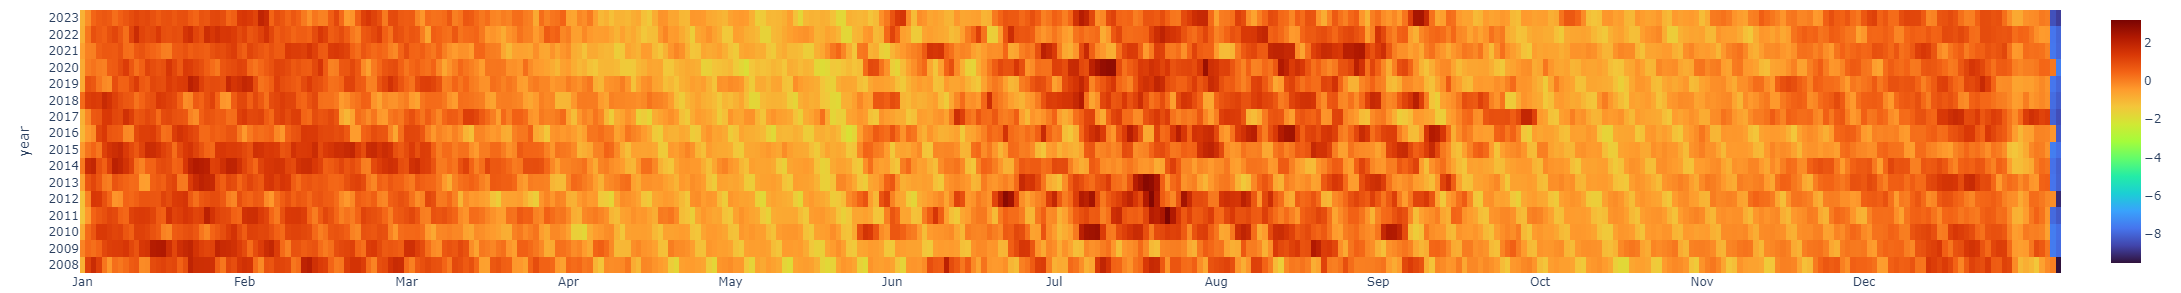
\includegraphics[height=3.75cm]{figures/seasonality.png}
    \caption{Seasonality of Daily energy consumption in Toronto (IESO, 2008-2023)}
  \end{figure}

  \end{block}

  \begin{block}{Approach}
    {\justifying
      The solution consists of 4 components: Dataset Builder API, Forecasting Models, an Anomaly Detection Model, and an Interactive Dashboard. The user can choose the entire dataset or a subset of it to build the dataset and train the model. The results are then visualized using the dashboard.
    }

    \begin{figure}
      \centering
      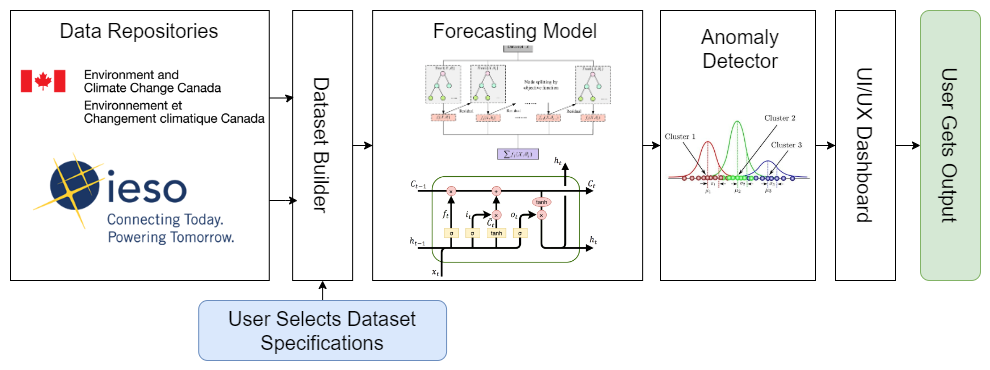
\includegraphics[height=10.0cm]{figures/system_arch.png}
      \caption{Full System Architecture}
    \end{figure}

    \subheading{Forecasting Models: XGBoost}\\
    {\justifying
      Forecasting module 1 leverages \textbf{XGBoost (Extreme Gradient Boosting)} to forecast daily energy demand based on historical consumption patterns and weather features such as temperature and humidity. XGBoost was chosen because it is a tree-based ensemble learning algorithm known for its speed and performance and interpretability. 
    }

    \begin{figure}
      \centering
      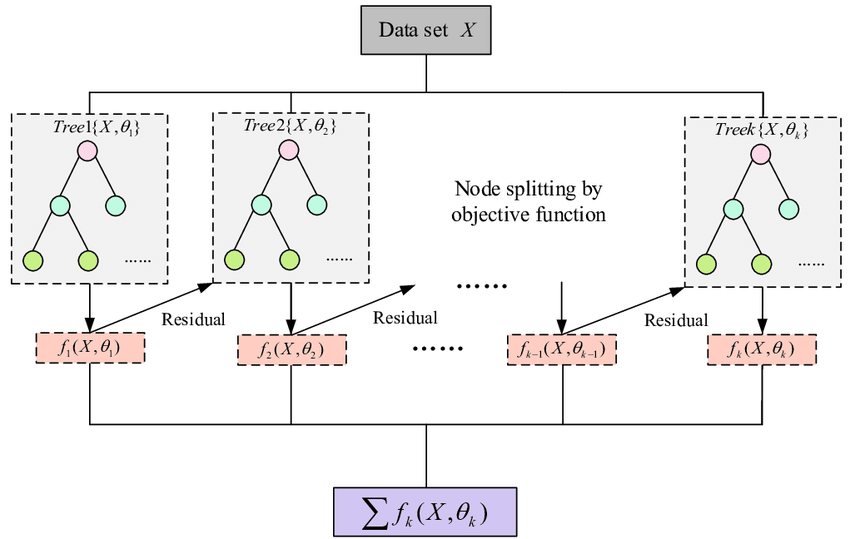
\includegraphics[height=8.5cm]{figures/xgboost.png}
      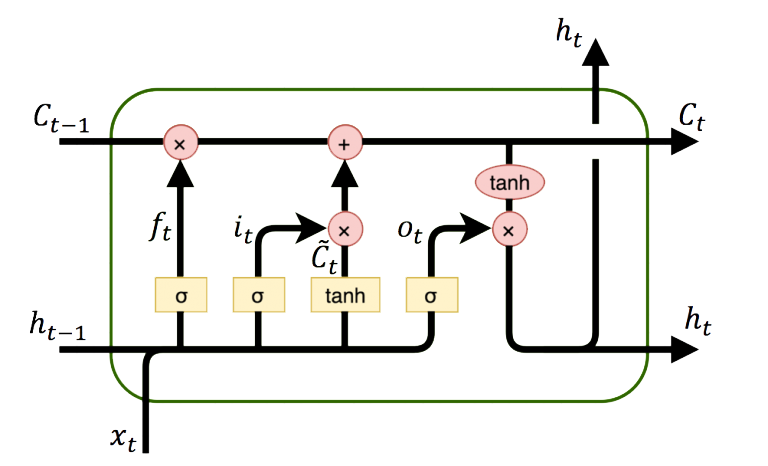
\includegraphics[height=8.0cm]{figures/lstm.png}
      \caption{Model Architectures for XGBoost (left) and LSTM (right)}
    \end{figure}

  \end{block}



% column 2
\end{column}
\separatorcolumn
\begin{column}{\colwidth}

  \subheading{Forecasting Models: LSTM}\\
    {\justifying
      Forecasting module 2 uses \textbf{LSTM (Long Short-Term Memory)}, which are Recurrent Neural Networks (RNN) designed to handle sequential data. LSTMs are highly effective for time-series forecasting as they address the vanishing gradient problem using memory cells and information gates.
    } 

  \subheading{Anomaly Detection Model}\\
  \begin{figure}
    \centering
    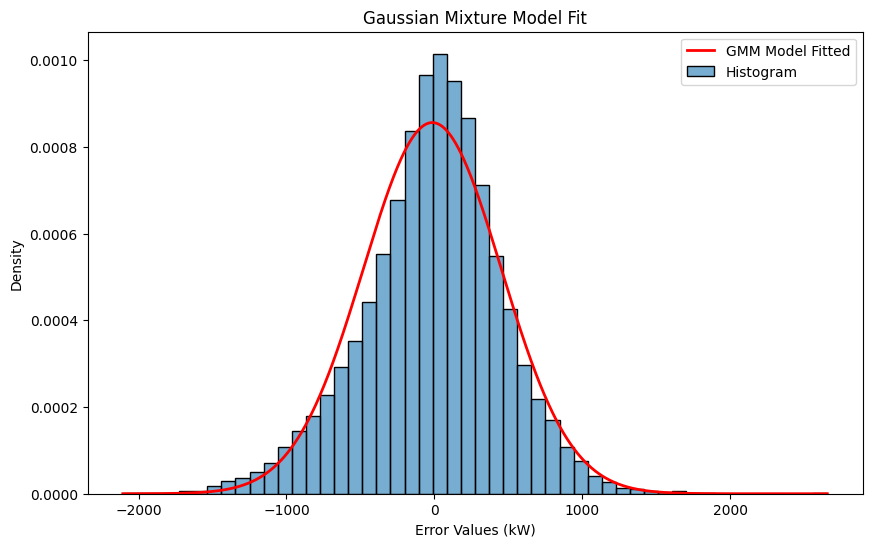
\includegraphics[height=8.75cm]{figures/gmm.png}
    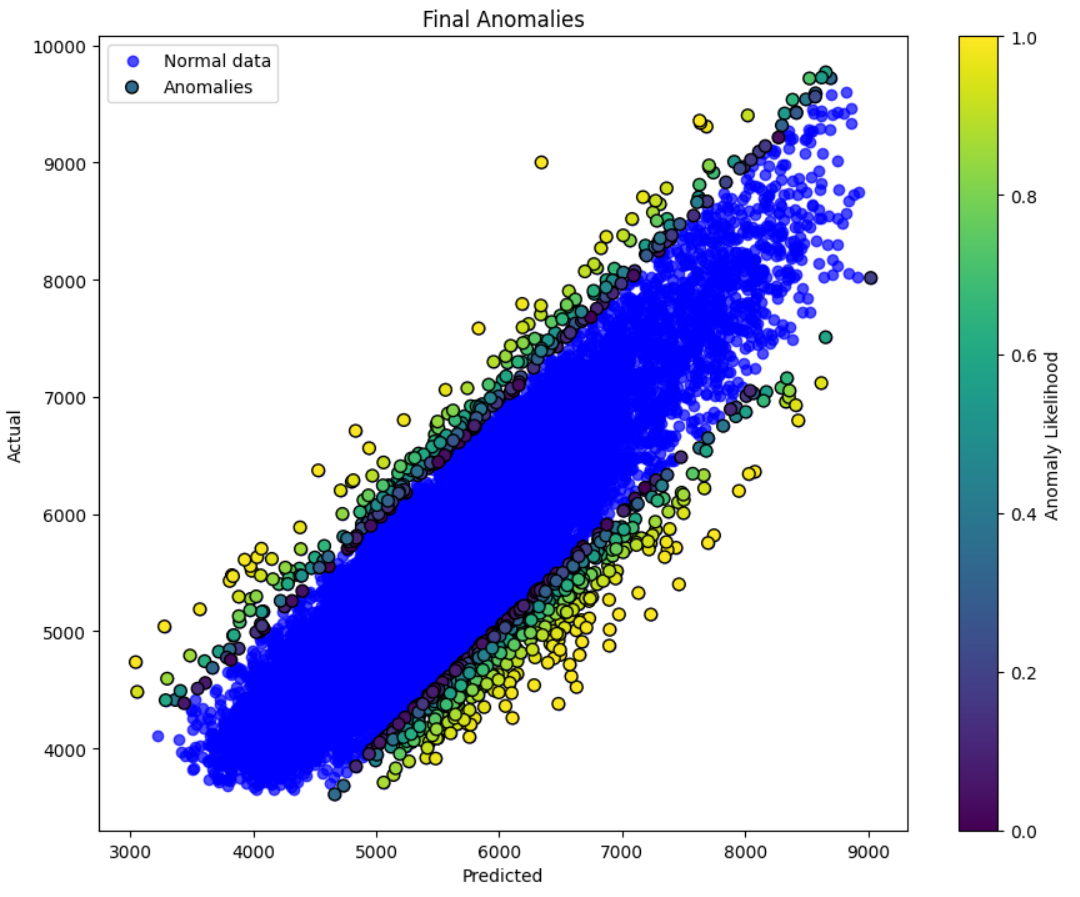
\includegraphics[height=8.75cm]{figures/ad.png}
    \caption{Gaussian Mixture Model fit (left) and Anomaly Detection Model output (right)}
  \end{figure}
  {\justifying
    The \textbf{Anomaly Detection (AD)} module employs statistical and probabilistic models of the error between the predicted and actual energy demand. \textbf{Gaussian Mixture Modelling (GMM)} with \textbf{Expectation-Maximization (EM)} algorithm is used for unsupervised latent state modelling to determine the likelihood that a prediction error belongs to or falls outside of an expected distribution of errors.
  }

  \subheading{Interactive Dashboard}\\
  The dashboard is a web/local application that allows the user to interact with the forecasting and anomaly detection models. The dashboard allow convenient training and inference of the models. Moreover, the user can bring their own data to train the model and test the results for anomalies.

  \vspace{0.25cm}
  \begin{block}{Results}

    \begin{figure}
      % \centering
      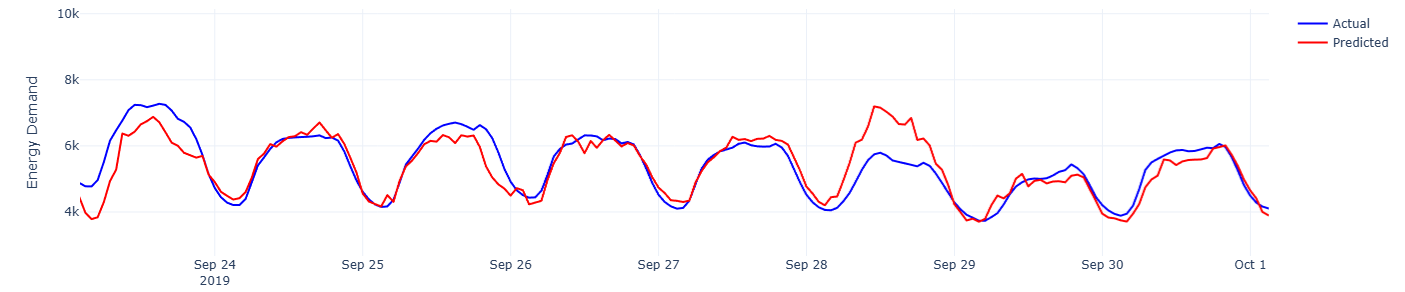
\includegraphics[height=5.5cm]{figures/xgb-pred.png}
      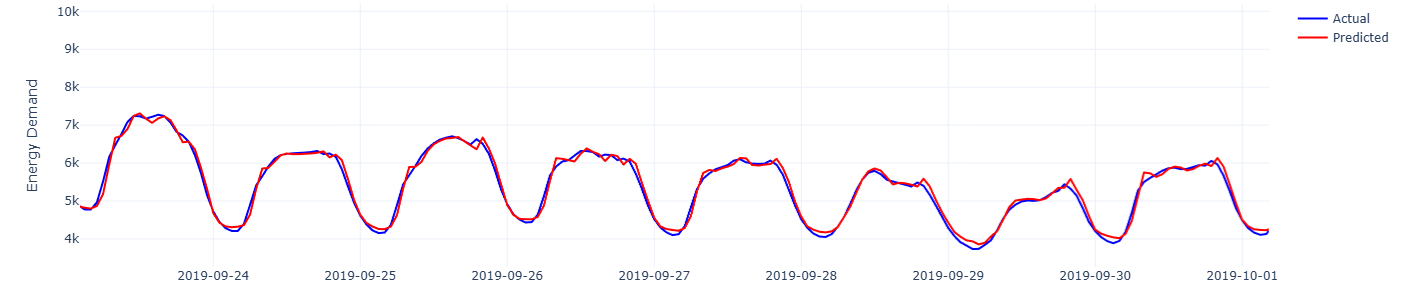
\includegraphics[height=5.5cm]{figures/lstm-pred.png}
      \caption{Hourly energy demand predictions of XGBoost (top) and LSTM (bottom) based on energy and weather data (Toronto Zonal, 2018-2021)}
    \end{figure}

    \vspace{-0.5cm}
    The models were evaluated on multiple datasets from IESO, including both Zonal (aggregated) and Forward Sortation Area (FSA) level data. % The models demonstrated strong performance across different geographical scales, with LSTM generally achieving better accuracy than XGBoost. % For anomaly detection, we found that using a 3-component GMM provided the best balance between sensitivity and specificity in identifying unusual consumption patterns.

    \begin{table}
      \centering
      \vspace{-0.5cm}
      \caption{Model performance results on multiple datasets (from 2018–2020)}
      \begin{tabular}{l cc cc c}
        \toprule
        \multirow{2}{*}{\textbf{Models}} & \multicolumn{2}{c}{\textbf{Zonal}} & \multicolumn{2}{c}{\textbf{FSA}} & \multirow{2}{*}{\textbf{Num (Datasets)}} \\
        & \textbf{MAPE} & \textbf{Anom. \%} & \textbf{MAPE} & \textbf{Anom. \%} & \\
        \midrule
        XGBoost & 8.83\% & 4.70\% & 7.63\% & 5.0\% & 5 \\
        LSTM & 2.44\% & 2.33\% & 4.80\% & 4.69\% & 5 \\
        \bottomrule
      \end{tabular}
    \end{table}
  
  \end{block}
  \vspace{-0.5cm}
  \begin{block}{Conclusion}
  Our research demonstrates successful implementation of energy demand forecasting and anomaly detection using advanced machine learning models. The LSTM model achieved superior performance with MAPE of \textbf{2.44\%} on zonal data, while XGBoost showed robust results with \textbf{8.83\%} MAPE. With our interaactive dashboards, our work can contribute to efficient energy management by making these advanced tools more accessible.

  \end{block}
  \vspace{-0.5cm}
  \begin{block}{Acknowledgements}
  We would like to thank our supervisor, \textbf{Dr. Bala Venkatesh}, for his support throughout this project. We would also like to thank \textbf{Shima B.Z. Homayie} and \textbf{Amir R.N. Ghadikolaei} for their help and feedback.
  \end{block}

\end{column}


\end{columns}
\end{frame}

\end{document}
